% Entregable 4. Fuente única. Compilar: tectonic presentacion.tex
% Rediseño visual: fotografía real, capturas propias, iconos Lucide y fuentes OFL.
\documentclass[aspectratio=169,11pt]{beamer}
\usepackage{fontspec}
\setsansfont{dm-sans-400.ttf}[Path=recursos/fuentes/,BoldFont=dm-sans-700.ttf]
\setmainfont{dm-sans-400.ttf}[Path=recursos/fuentes/,BoldFont=dm-sans-700.ttf]
\newfontfamily\Body{dm-sans-400.ttf}[Path=recursos/fuentes/,BoldFont=dm-sans-700.ttf]
\newfontfamily\Display{barlow-condensed-700.ttf}[Path=recursos/fuentes/,BoldFont=barlow-condensed-700.ttf]
\usepackage[spanish]{babel}
\usepackage{tikz,graphicx,etoolbox}
\usetikzlibrary{arrows.meta,calc,positioning}
\usefonttheme{professionalfonts}
\setbeamertemplate{navigation symbols}{}\setbeamertemplate{headline}{}\setbeamertemplate{footline}{}
\setbeameroption{hide notes}\hyphenpenalty=10000\exhyphenpenalty=10000
\definecolor{Paper}{HTML}{F4F0E8}\definecolor{Ink}{HTML}{14332D}
\definecolor{Muted}{HTML}{5B6F67}\definecolor{Accent}{HTML}{327A6B}
\definecolor{Soft}{HTML}{E1E8DC}\definecolor{Line}{HTML}{D1D9D0}
\definecolor{White}{HTML}{FFFFFF}\definecolor{Night}{HTML}{10241F}
\definecolor{Mint}{HTML}{B7DBC1}\definecolor{Dull}{HTML}{A5BFB4}
\title[ATLAS MTB]{Desarrollo de una plataforma web para la selección, comparación y configuración tridimensional de bicicletas de montaña}
\author{Joel Ito Luque}\date{21 de octubre de 2026}
\hypersetup{pdfsubject={Gestión de Proyectos: presentación visual de 12 diapositivas}}
\newcommand{\tx}[6]{\node[anchor=north west,inner sep=0,align=left,text width=#3cm,text=#5,font=\Body\fontsize{#4}{\dimexpr #4pt+3pt\relax}\selectfont]at(#1,#2){#6};}
\newcommand{\hd}[6]{\node[anchor=north west,inner sep=0,align=left,text width=#3cm,text=#5,font=\Display\fontsize{#4}{\dimexpr #4pt+2pt\relax}\selectfont]at(#1,#2){#6};}
\newcommand{\canvas}[1]{\transfade[duration=.25]\begin{tikzpicture}[remember picture,overlay,shift={(current page.south west)}]
\ifstrequal{#1}{dark}{\colorlet{Bg}{Night}\colorlet{Fg}{White}\colorlet{Dim}{Dull}\colorlet{Hi}{Mint}}{\colorlet{Bg}{Paper}\colorlet{Fg}{Ink}\colorlet{Dim}{Muted}\colorlet{Hi}{Accent}}
\fill[Bg](0,0)rectangle(16,9);}
\newcommand{\header}[2]{\tx{.7}{8.54}{14.6}{7.4}{Hi}{#1}\hd{.7}{7.99}{14.6}{23}{Fg}{#2}}
\newcommand{\source}[1]{\tx{.7}{.92}{14.6}{5.5}{Dim}{#1}}
\newcommand{\finish}{\fill[Bg](0,0)rectangle(16,.62);\draw[Hi,opacity=.3](.7,.59)--(15.3,.59);\pgfmathsetmacro{\progress}{.7+14.6*\insertframenumber/12}\draw[Hi,line width=1pt](.7,.59)--(\progress,.59);\tx{.7}{.38}{12.8}{5.8}{Dim}{ATLAS MTB\quad /\quad GESTIÓN DE PROYECTOS\quad /\quad 21 OCT 2026}\tx{14.5}{.38}{.9}{5.8}{Dim}{\insertframenumber\,/\,12}\end{tikzpicture}}
\newcommand{\ico}[5]{\node[anchor=north west,inner sep=0]at(#2,#3){\includegraphics[width=#4cm]{recursos/iconos/#1-#5.png}};}
% Iconos Lucide (ISC): fuentes SVG y PNG de 192 px incluidos en recursos/iconos/.

\begin{document}
% 1. Portada · fotografía real
\begin{frame}[plain]
\canvas{dark}
\begin{scope}\clip(0,0)rectangle(16,9);\node[inner sep=0]at(11.45,4.6){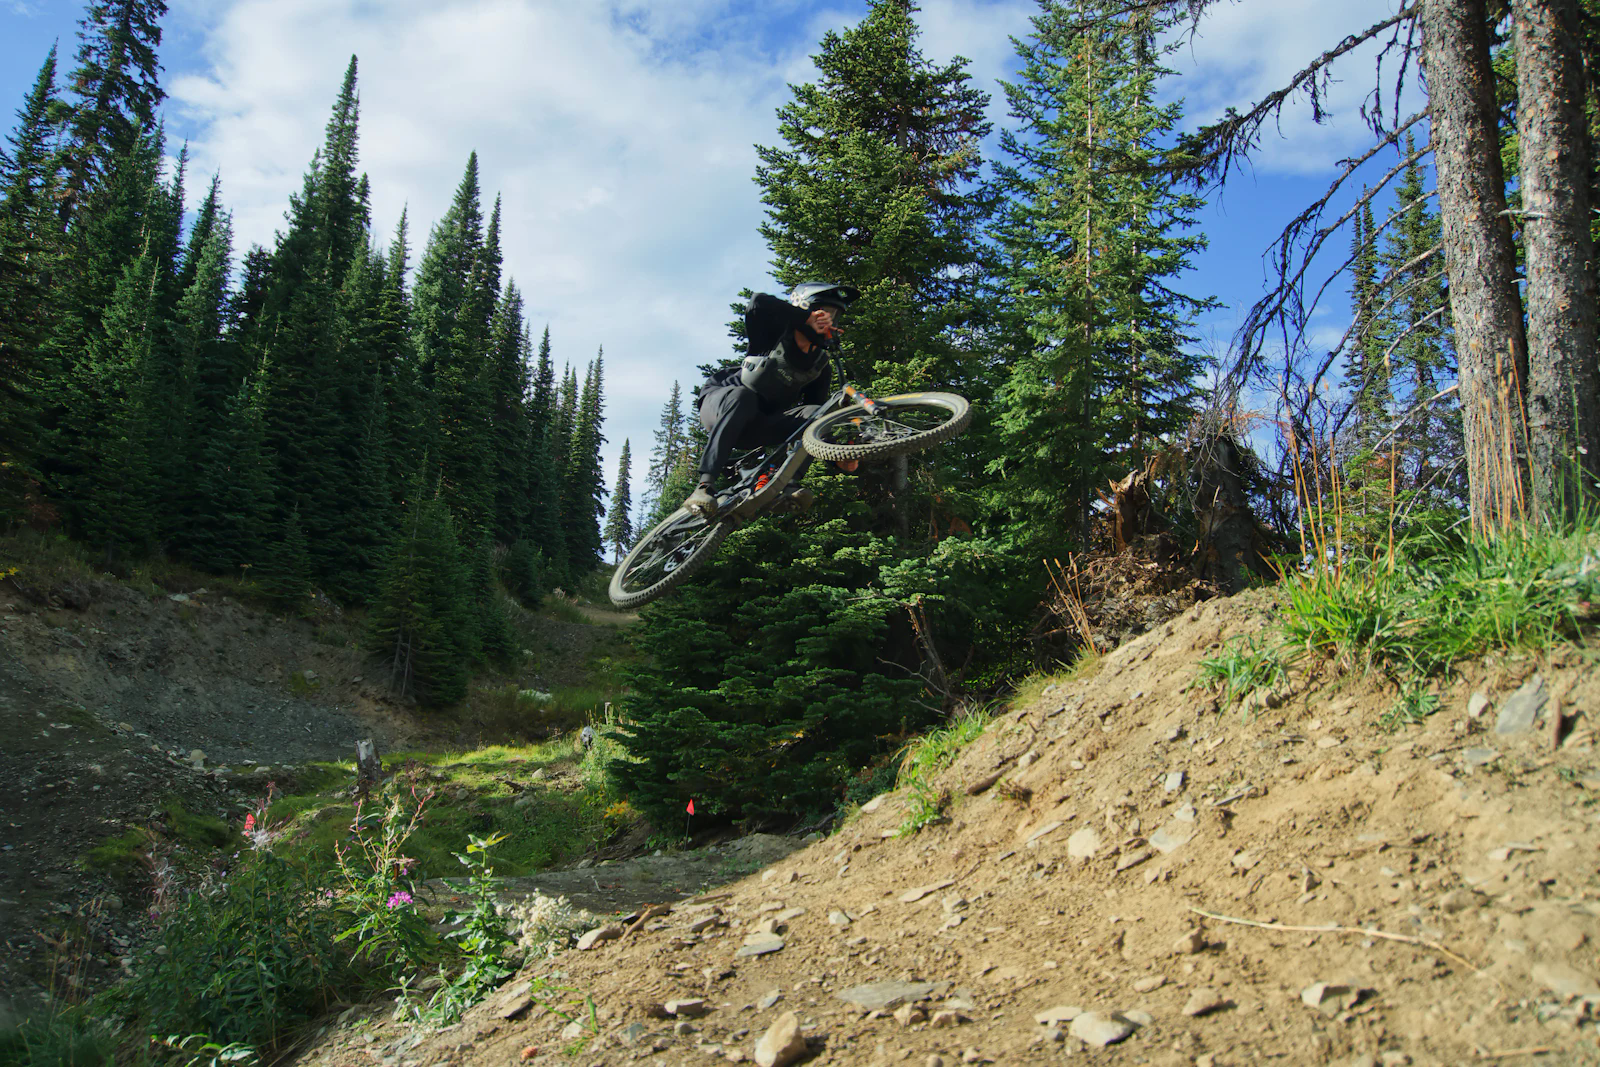
\includegraphics[width=16cm]{recursos/mtb-accion.png}};\end{scope}
\fill[Night](0,0)--(8.45,0)--(7.1,9)--(0,9)--cycle;\draw[Mint,opacity=.5,line width=.5pt](7.1,9)--(8.45,0);

\tx{.7}{8.45}{6.2}{7.5}{Mint}{GESTIÓN DE PROYECTOS / INDIVIDUAL}
\hd{.65}{7.95}{7}{39}{White}{ATLAS MTB}
\fill[Mint](.7,6.35)rectangle(1.5,6.41);
\hd{.7}{6.03}{6.4}{12.2}{White}{Desarrollo de una plataforma web\\para la selección, comparación y\\configuración tridimensional\\de bicicletas de montaña}
\tx{.7}{3.55}{6.2}{11}{Mint}{\bfseries Joel Ito Luque}
\tx{.7}{2.92}{6.45}{7.4}{White}{Universidad Nacional de Juliaca\\Facultad de Ciencias de la Ingeniería\\Ingeniería de Software y Sistemas}
\tx{.7}{1.76}{6.5}{6.8}{White}{Docente: Fidel Huanco Ramos · Octavo semestre\\Juliaca, Perú · 21 de octubre de 2026}
\fill[Night,opacity=.55](8.95,.72)rectangle(15.35,1.05);\tx{9.1}{.96}{6.2}{5.5}{White}{Foto: \href{https://unsplash.com/photos/534Moyd3Lf4}{Julien Kettmann / Unsplash} · Sun Peaks, Canadá}
\finish
\note{Presenta una web para consultar piezas, explorar un montaje y guardarlo. La fotografía real de acción contextualiza el deporte; no es un montaje generado por la aplicación. Autor de la foto: Julien Kettmann, Unsplash. El trabajo es individual. Mantén el título académico completo y explica ATLAS MTB como nombre del software. Tiempo: 35 segundos.}
\end{frame}

% 2. Problema · piezas de información dispersas
\begin{frame}[plain]
\canvas{light}\header{01 / PROBLEMA Y JUSTIFICACIÓN}{El problema: planificación fragmentada}
\tx{.85}{6.8}{7}{10}{Muted}{Al armar o modificar una bicicleta}
\begin{scope}[shift={(1.1,2.4)},rotate=7]
\filldraw[fill=White,draw=Line,rounded corners=3pt](0,0)rectangle(3.5,3.6);
\ico{layers}{.35}{3.23}{.65}{Accent}\hd{.35}{2.25}{2.8}{17}{Ink}{FICHAS}
\foreach \y/\w in {1.55/2.6,1.15/1.8,.75/2.2}{\draw[Line,line width=2pt](.35,\y)--++(\w,0);}
\end{scope}
\begin{scope}[shift={(3.6,1.9)},rotate=-6]
\filldraw[fill=Soft,draw=Line,rounded corners=3pt](0,0)rectangle(3.5,2.8);
\ico{ruler}{.35}{2.45}{.6}{Accent}\hd{.35}{1.55}{2.8}{19}{Ink}{29 / 27,5}
\tx{.35}{.67}{2.8}{9}{Muted}{Medidas y versiones}
\end{scope}
\draw[Accent,line width=1pt,dashed,-{Latex[length=2mm]}](7.7,3.8)to[bend left=18](9.05,4.8);
\hd{8.9}{6.35}{6.3}{20}{Ink}{CONSULTAS\\DESCONECTADAS}
\tx{8.9}{4.65}{6.3}{10}{Muted}{Las piezas y sus variantes se consultan por separado, sin una visión integrada del montaje.}
\tx{8.9}{2.65}{6.3}{9}{Ink}{Dificulta relacionar elecciones y retomar una propuesta.}
\hd{.8}{1.48}{14.2}{13}{Accent}{Justificación: integrar consulta, comparación y montaje.}
\source{Fuentes: \href{https://productinfo.shimano.com/en/compatibility}{compatibilidad técnica 1} · \href{https://www.sram.com/en/service/manuals--documents/compatability-map}{compatibilidad técnica 2}. Problema de planificación; sin estudio de campo.}
\finish\note{El problema general del informe es cómo facilitar la planificación del armado o modificación de bicicletas mediante selección, comparación y visualización integrada. Aquí se concreta en la falta de continuidad cuando se consultan piezas y se anotan elecciones por separado: cuesta relacionar variantes, imaginar el conjunto y retomar la propuesta. Por ejemplo, elegir un aro también exige revisar el neumático y sus medidas. La justificación es integrar esas tareas en un mismo recorrido. Corresponde a los apartados 1.2, 1.3 y 1.4 del informe y al punto 2 de la consigna de presentación. No afirmes que se encuestó a ciclistas, que nadie ofrece soluciones parecidas ni que se midió un ahorro. Tiempo: 60 segundos.}
\end{frame}

% 3. Solución · escena real del software
\begin{frame}[plain]
\canvas{dark}\header{02 / SOLUCIÓN Y OBJETIVOS}{Explorar el montaje completo}
\begin{scope}\clip[rounded corners=5pt](5.55,1.75)rectangle(15.35,6.7);\node[inner sep=0]at(10.45,4.25){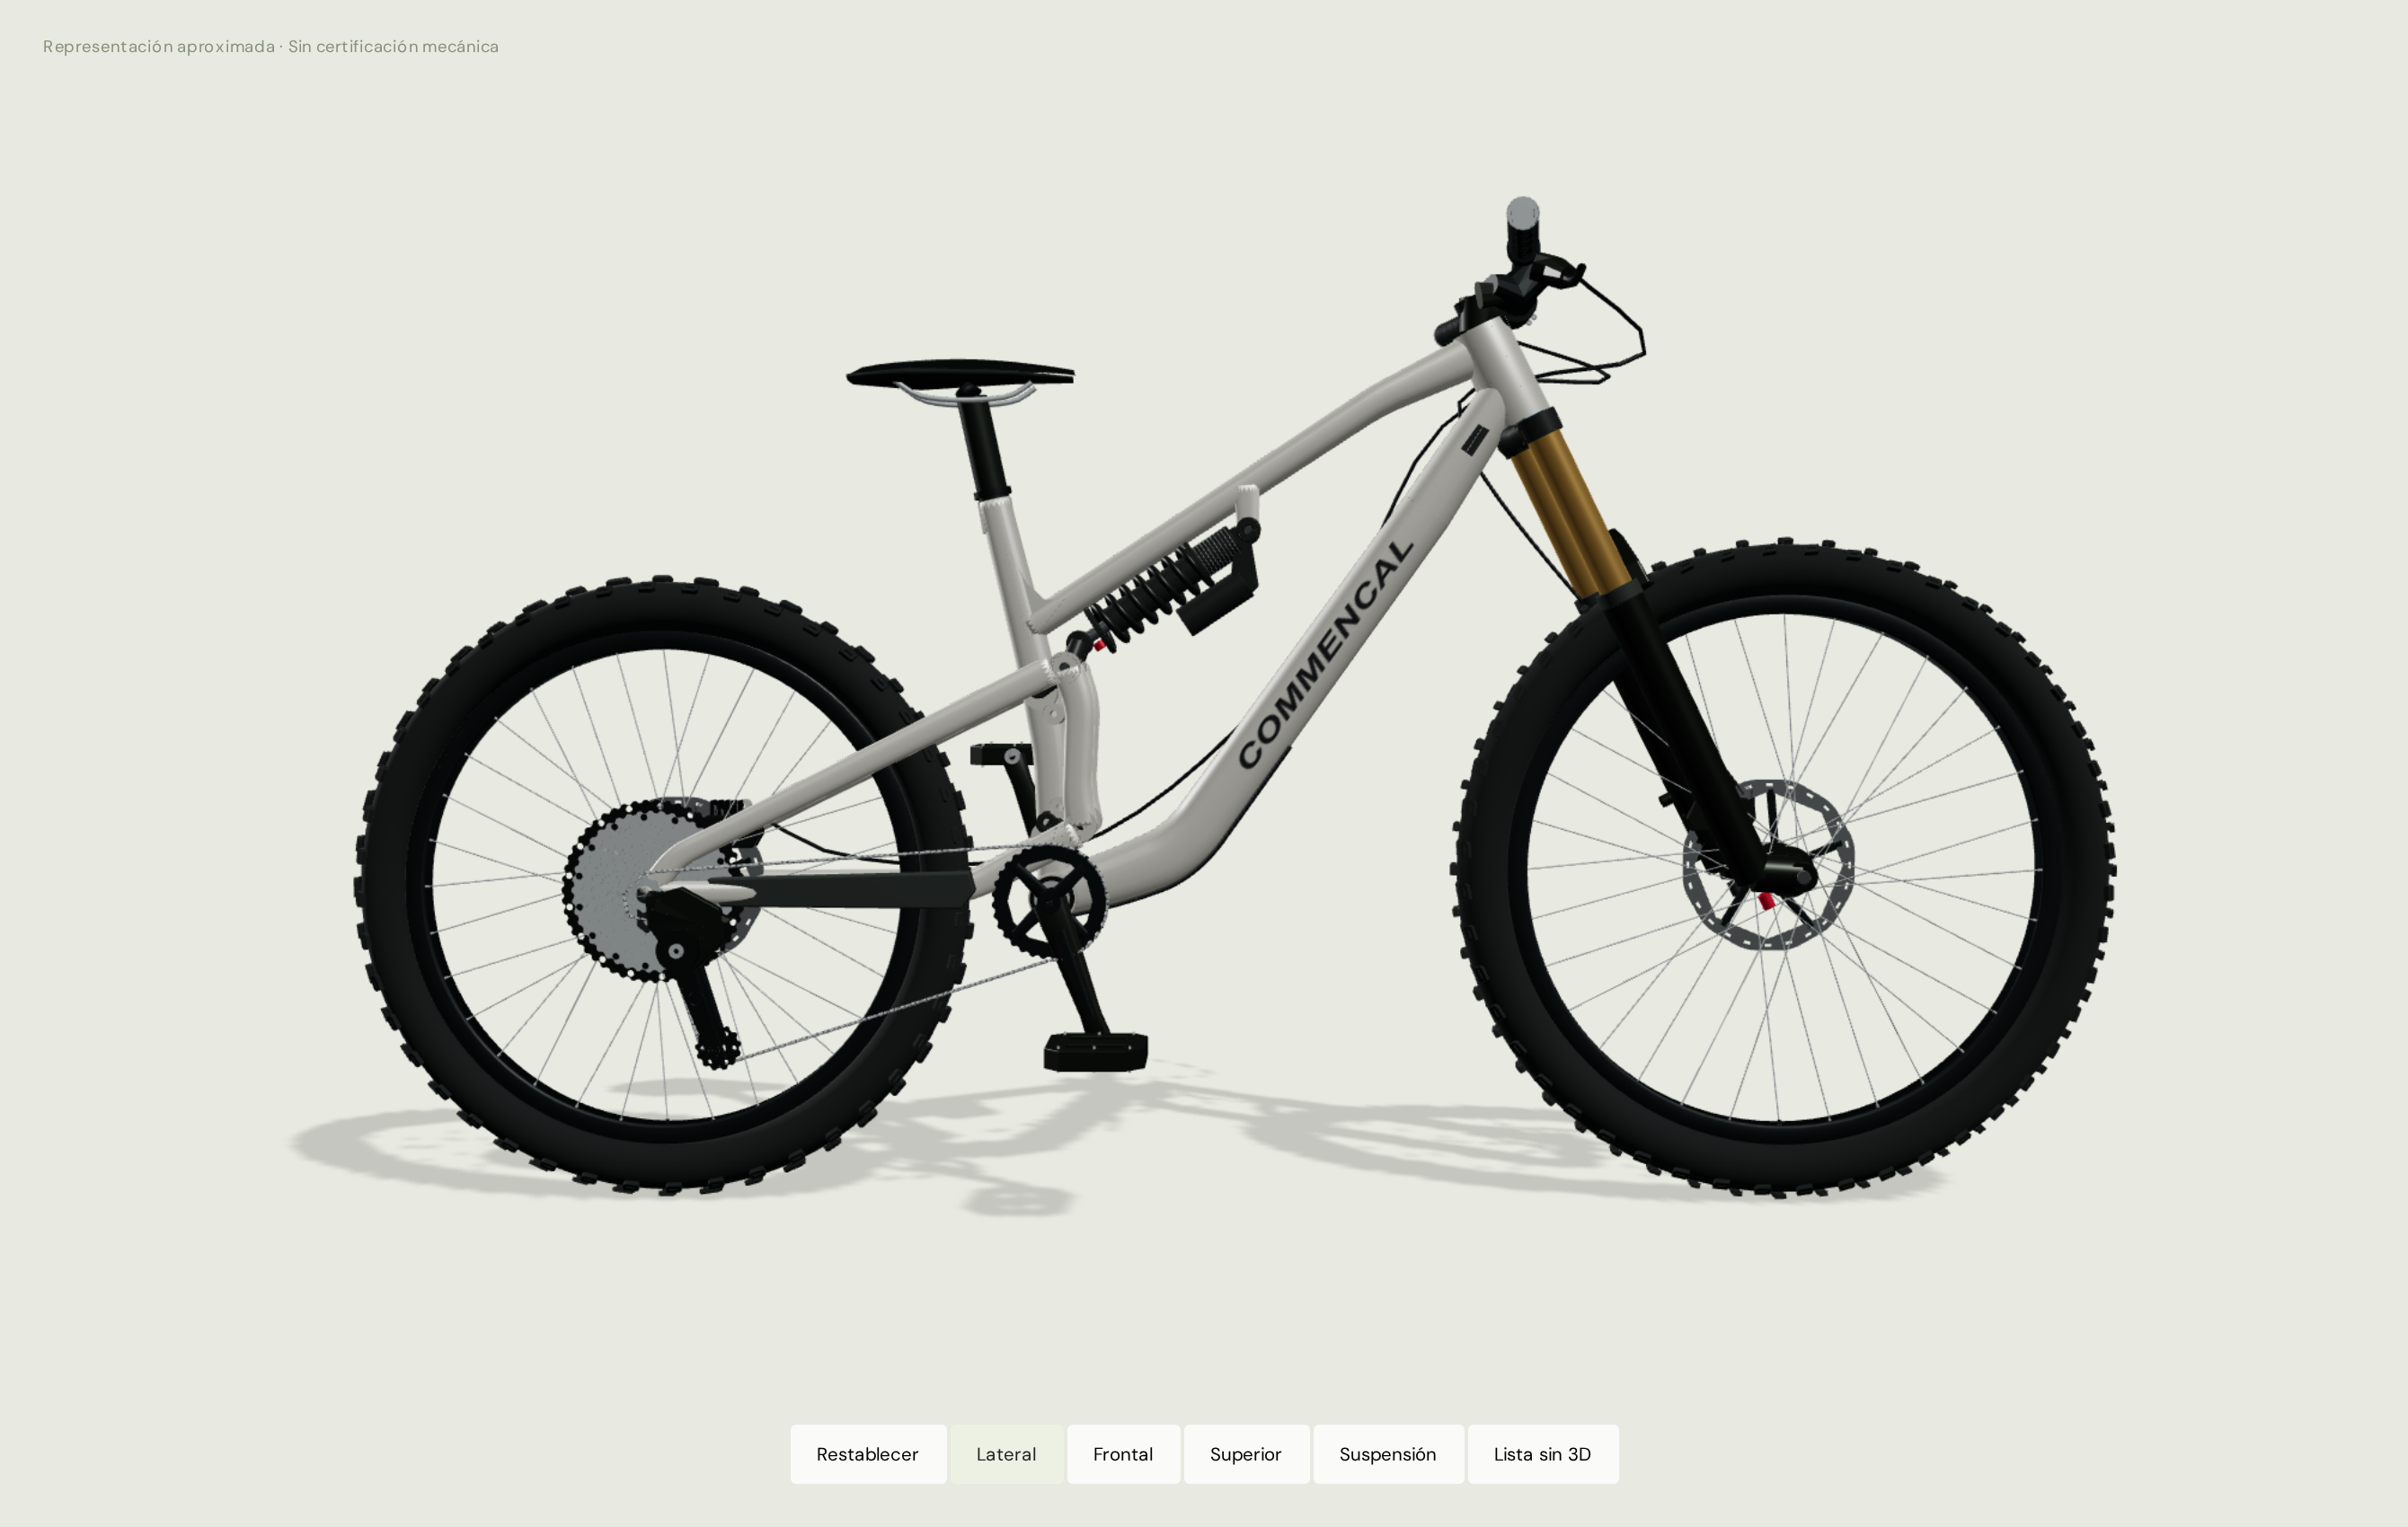
\includegraphics[width=10.3cm]{recursos/montaje-lateral.png}};\end{scope}
\foreach \y/\n/\icon/\label in {6.4/01/search/CONSULTAR,4.85/02/git-compare-arrows/COMPARAR,3.3/03/save/GUARDAR}{
\tx{.8}{\y}{.6}{7}{Mint}{\n}\ico{\icon}{1.55}{\y+.08}{.65}{Mint}\hd{2.45}{\y+.08}{2.8}{18}{White}{\label}}
\tx{6}{1.48}{9.2}{8.5}{Mint}{Piezas + acabados + avisos del montaje}
\source{Captura real en vista lateral. Representación aproximada; no certificación mecánica. Objetivos completos: informe, sección 1.}
\finish\note{Relaciona cada objetivo con una acción: consultar antes de elegir, explorar un conjunto y conservar una propuesta. La imagen es una captura real del visor en vista lateral. La aplicación orienta la planificación; no certifica que una combinación sea físicamente compatible ni sustituye a un especialista. Los objetivos completos están en el informe: catálogo, configurador, acceso y persistencia, administración y validación. Tiempo: 60 segundos.}
\end{frame}

% 4. Alcance · mapa de funciones
\begin{frame}[plain]
\canvas{light}\header{03 / ALCANCE}{Todo parte de tu montaje}
\draw[Line,line width=.8pt](7.9,4.55)ellipse(4.6 and 1.65);
\fill[Ink](7.9,4.55)circle(.8);\ico{layers}{7.45}{5.04}{.9}{Mint}
\foreach \x/\y/\icon/\label in {3.2/5.9/search/Catálogo,7.9/6.35/git-compare-arrows/Comparación,12.6/5.9/scan-line/Configuración,3.2/3.2/save/Mis bicicletas,7.9/2.95/user-round/Acceso,12.6/3.2/shield-check/Administración}{
\fill[Paper](\x,\y)circle(.53);\ico{\icon}{\x-.3}{\y+.3}{.6}{Accent}
\node[anchor=north,font=\Body\fontsize{10}{13}\selectfont,text=Ink]at(\x,\y-.65){\label};}
\hd{.85}{1.63}{3}{14}{Ink}{4 ENTREGABLES}
\ico{code-xml}{4.2}{1.56}{.38}{Accent}\tx{4.8}{1.53}{2}{8}{Muted}{Software}
\ico{folder}{7}{1.56}{.38}{Accent}\tx{7.6}{1.53}{1.9}{8}{Muted}{Informe}
\ico{layers}{9.7}{1.56}{.38}{Accent}\tx{10.3}{1.53}{1.8}{8}{Muted}{Manual}
\ico{monitor}{12.3}{1.56}{.38}{Accent}\tx{12.9}{1.53}{2.4}{8}{Muted}{Presentación}
\source{23 posiciones · comparación de hasta tres variantes · acciones por permiso. Sin compras ni pagos. Fuente: informe, sección 1.}
\finish\note{Explica el alcance como seis capacidades conectadas. La comparación se limita a variantes de una misma categoría. Las 23 posiciones son espacios de montaje, no 23 productos distintos del catálogo. La administración tiene permisos explícitos y el registro público no otorga privilegios. La entrega académica tiene cuatro productos; la presentación no reemplaza al código o al manual. Tiempo: 55 segundos. El mapa reúne seis funciones alrededor del montaje; las cuatro salidas inferiores son entregables académicos.}
\end{frame}

% 5. Cronograma · Gantt
\begin{frame}[plain]
\canvas{light}\header{04 / GESTIÓN DEL TIEMPO}{Tres semanas de integración y cierre}
\foreach \x/\n/\date in {5.35/01/30 sep–6 oct,8.65/02/7–13 oct,11.95/03/14–20 oct}{
\hd{\x}{6.78}{1.2}{25}{Accent}{\n}\tx{\x+1.05}{6.38}{2.15}{8}{Muted}{\date}}
\foreach \label/\start/\stop/\row in {Análisis y diseño/1/5/0,Datos y acceso/4/7/1,Catálogo y comparación/6/10/2,3D y montaje/4/14/3,Gestión y administración/10/15/4,Interacción y acabados/13/16/5,Pruebas y correcciones/7/20/6,Preparar publicación/19/21/7}{
\pgfmathsetmacro{\yy}{5.38-.46*\row}
\tx{.85}{\yy+.12}{4.25}{9.2}{Ink}{\label}
\draw[Line,line width=.3pt](5.35,\yy-.15)--(15.2,\yy-.15);
\pgfmathsetmacro{\xa}{5.35+(\start-1)*.469}\pgfmathsetmacro{\xb}{5.35+\stop*.469}
\fill[Accent,rounded corners=1.1pt](\xa,\yy+.09)rectangle(\xb,\yy-.09);}
\foreach \x in {8.633,11.916}{\draw[Line,dashed](\x,5.75)--(\x,1.96);}
\ico{user-round}{.85}{1.66}{.36}{Accent}\tx{1.4}{1.61}{8.8}{9}{Ink}{Joel Ito Luque · responsabilidad individual}
\ico{clock-3}{10.45}{1.66}{.36}{Accent}\tx{11}{1.61}{4.2}{9}{Muted}{Actividades solapadas}
\source{Estimación reconstruida 30/09–20/10/2026, desde un prototipo previo; no registro real de ejecución. Detalle: informe, sección 2.}
\finish\note{Aclara que las tres semanas son una reconstrucción estimada de integración y cierre a partir de un prototipo; no representan todo el desarrollo desde cero ni un registro horario real. Las barras agrupan actividades del Gantt del informe y mantienen sus intervalos. Señala que pruebas y preparación 3D se solapan con implementación. El último bloque es preparación de publicación, sin atribuir una fecha real de despliegue no demostrada. Tiempo: 65 segundos.}
\end{frame}

% 6. Recursos y riesgos · iconos semánticos
\begin{frame}[plain]
\canvas{light}\header{05 / RECURSOS Y RIESGOS}{Una persona, tres frentes de control}
\fill[Ink,rounded corners=5pt](.7,2.0)rectangle(4.5,6.7);
\ico{user-round}{1.85}{6.15}{1.45}{Mint}
\hd{1.05}{4.5}{3.1}{18}{White}{JOEL ITO\\LUQUE}
\tx{1.05}{2.9}{3.1}{7.2}{Mint}{Análisis · desarrollo\\Pruebas · documentación}
\foreach \y/\icon/\risk/\resp in {6.3/database/Datos incompletos/Fuentes,4.8/shield-check/Acceso indebido/Permisos,3.3/gauge/Carga del visor/Modo lista}{
\ico{\icon}{5.15}{\y}{.7}{Accent}\hd{6.15}{\y-.05}{4.1}{17}{Ink}{\risk}
\draw[-{Latex[length=2mm]},Accent,line width=.8pt](10.8,\y-.35)--(11.7,\y-.35);
\tx{12.1}{\y-.14}{3.1}{11}{Muted}{\resp}}
\ico{monitor}{.85}{1.6}{.4}{Accent}\tx{1.5}{1.52}{3.8}{8.5}{Muted}{Equipo personal}
\ico{code-xml}{5.8}{1.6}{.4}{Accent}\tx{6.45}{1.52}{3.8}{8.5}{Muted}{Herramientas}
\ico{cloud}{10.9}{1.6}{.4}{Accent}\tx{11.55}{1.52}{3.8}{8.5}{Muted}{Servicios en nube}
\source{Respuestas de gestión, no garantía de ausencia de riesgos. Fuente: informe, sección 2.}
\finish\note{Presenta la responsabilidad individual sin inventar miembros de equipo. Explica tres riesgos: datos insuficientes se responden conservando fuentes y distinguiendo lo conocido; acceso indebido se limita con permisos y propiedad; carga gráfica se atiende con recursos optimizados y una alternativa sin 3D. Estas respuestas no eliminan todos los riesgos. Se emplearon equipo personal y servicios en nube; no se inventó presupuesto ni dedicación horaria medida. Tiempo: 60 segundos.}
\end{frame}

% 7. Arquitectura · flujo sobre fondo oscuro
\begin{frame}[plain]
\canvas{dark}\header{06 / ARQUITECTURA}{La experiencia conectada a la nube}
\ico{globe}{1.2}{6.55}{.7}{Mint}\hd{2.2}{6.53}{4.4}{18}{White}{NETLIFY}
\tx{2.2}{5.88}{4.4}{9}{Dim}{Publicación HTTPS}
\draw[-{Latex[length=2mm]},Mint,line width=1pt](3.15,5.25)--(3.15,4.75);
\ico{monitor}{1.15}{4.55}{1.15}{Mint}\hd{2.7}{4.46}{3.6}{20}{White}{NAVEGADOR}
\tx{1.15}{2.95}{5.9}{10}{White}{React + TypeScript · Three.js}
\tx{1.15}{2.35}{5.9}{8.5}{Dim}{Reglas de montaje separadas del visor.}
\draw[{Latex[length=2mm]}-{Latex[length=2mm]},Mint,line width=1pt](6.65,4.15)--(8.15,4.15);
\tx{6.73}{4.88}{1.6}{7.2}{Dim}{Consulta\\y sesión}
\ico{cloud}{9.1}{6.48}{1.5}{Mint}\hd{11}{6.2}{4.3}{22}{White}{SUPABASE}
\tx{11}{5.39}{4.3}{10}{Dim}{Cloud}
\foreach \x/\y/\icon/\label in {9.15/4.4/user-round/Acceso,12.5/4.4/database/Datos,9.15/2.8/folder/Archivos,12.5/2.8/code-xml/Funciones}{
\ico{\icon}{\x}{\y}{.6}{Mint}\tx{\x+.85}{\y-.15}{2.35}{9}{White}{\label}}
\source{Las fotos del frontend se publican en Netlify; modelos importados y miniaturas en Storage. Fuente: arquitectura implementada.}
\finish\note{Explica tres responsabilidades. Netlify entrega el frontend. El navegador presenta la interfaz y dibuja la escena; las reglas se mantienen separadas de React, el visor y el servicio de datos. Supabase gestiona identidad, base, archivos y operaciones administrativas. La base sigue en Cloud tanto en desarrollo como en la web publicada. Las fotos incluidas en el frontend se sirven con Netlify; modelos importados y miniaturas se conservan en Storage. Tiempo: 70 segundos.}
\end{frame}

% 8. Datos · dos cadenas y sus referencias
\begin{frame}[plain]
\canvas{light}\header{07 / DISEÑO DE DATOS}{Conservar piezas, versiones y montajes}
\hd{.8}{6.45}{3.6}{68}{Accent}{12}
\hd{.9}{3.95}{3.4}{15}{Ink}{TABLAS PROPIAS}
\tx{.9}{3.05}{3.3}{10}{Muted}{8 de negocio\\4 de autorización}
\draw[Line](4.65,2.05)--(4.65,6.65);
\tx{5.2}{6.5}{9.7}{7.5}{Accent}{CATÁLOGO}
\foreach \x/\icon/\label in {5.35/boxes/Modelo,8.8/ruler/Variante,12.25/scan-line/Recurso 3D}{
\ico{\icon}{\x+.65}{5.85}{.75}{Accent}\hd{\x}{4.85}{2.8}{18}{Ink}{\label}}
\draw[-{Latex[length=2mm]},Accent](7.8,5.45)--(8.7,5.45);\draw[-{Latex[length=2mm]},Accent](11.2,5.45)--(12.1,5.45);
\tx{5.2}{3.9}{9.7}{7.5}{Accent}{GUARDADO PERSONAL}
\foreach \x/\icon/\label in {5.35/user-round/Cuenta,8.8/layers/Montaje,12.25/save/Selecciones}{
\ico{\icon}{\x+.65}{3.23}{.75}{Accent}\hd{\x}{2.23}{2.8}{18}{Ink}{\label}}
\draw[-{Latex[length=2mm]},Accent](7.8,2.84)--(8.7,2.84);\draw[-{Latex[length=2mm]},Accent](11.2,2.84)--(12.1,2.84);
\draw[-{Latex[length=1.7mm]},Accent,dashed](13.6,3.5)--(13.6,3.85)--(10.15,3.85)--(10.15,4.06);
\source{Esquema conceptual. Auth gestiona la identidad. Los guardados conservan variantes y acabados; no duplican toda la escena 3D.}
\finish\note{Distingue modelo de variante con un ejemplo genérico: el nombre agrupa opciones, pero las medidas pertenecen a una elección concreta. El recurso visual contiene el archivo o la descripción con que se dibuja. En el guardado se conservan posiciones, variantes y acabados, por lo que no se duplica un archivo 3D de toda la bicicleta. Auth gestiona la cuenta, que no se cuenta como una decimotercera tabla propia. Los montajes previos conservan sus versiones. Tiempo: 65 segundos.}
\end{frame}

% 9. Módulos · collage de controles reales
\begin{frame}[plain]
\canvas{light}\header{08 / IMPLEMENTACIÓN}{Tres espacios, un mismo recorrido}
\fill[Soft,rounded corners=4pt](.7,1.65)rectangle(4.5,6.6);
\begin{scope}\clip(.95,2.3)rectangle(4.25,6.3);\node[anchor=north,inner sep=0]at(2.6,6.3){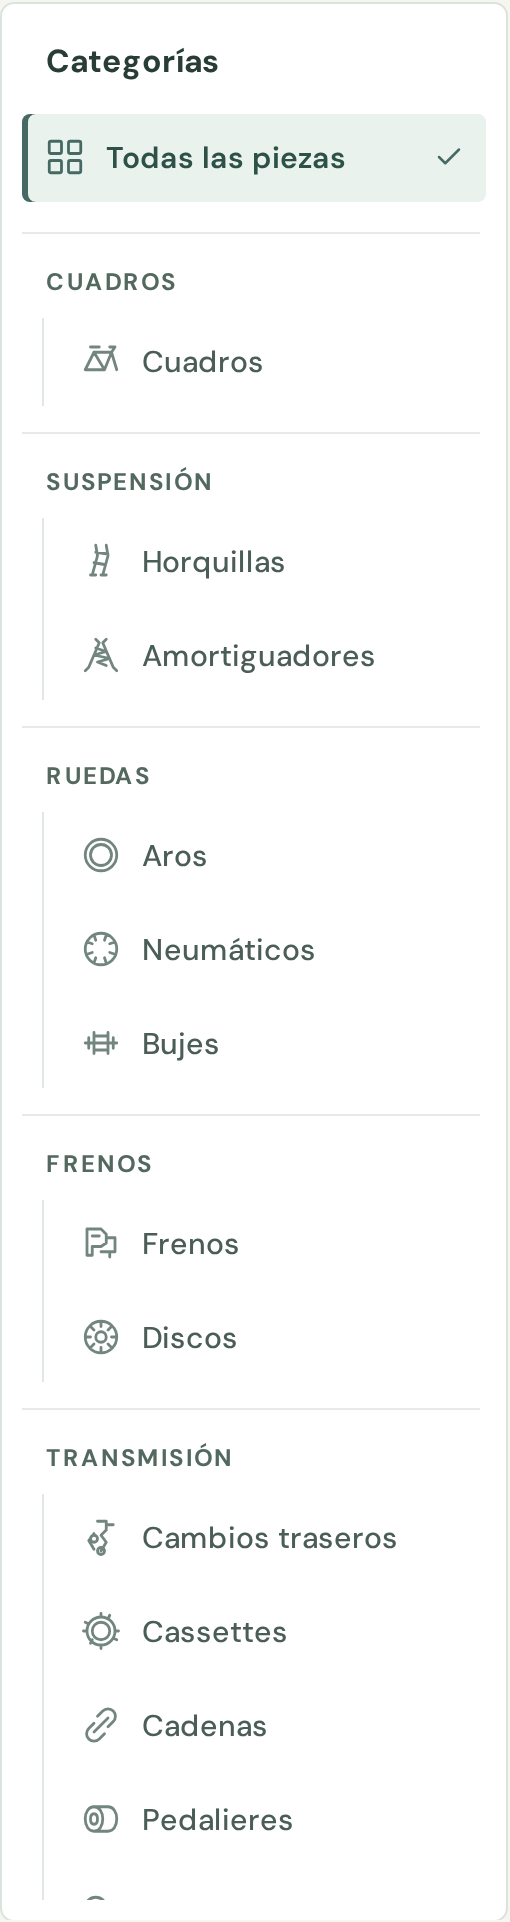
\includegraphics[width=3.3cm]{recursos/05-categorias.png}};\end{scope}
\hd{1}{2.17}{3.2}{19}{Ink}{EXPLORA}
\fill[White,rounded corners=4pt](4.95,2.2)rectangle(10.6,6.6);
\node[anchor=north,inner sep=0]at(7.78,6.28){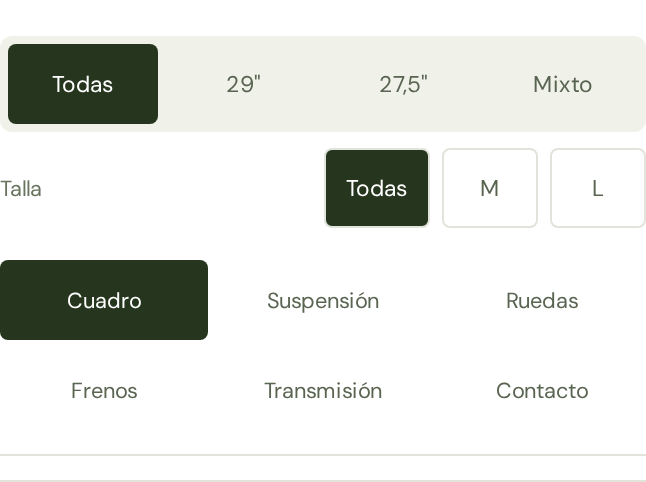
\includegraphics[width=4.8cm]{recursos/07-grupos-talla.png}};
\begin{scope}\clip(5.4,2.3)rectangle(10.2,2.9);\node[anchor=north,inner sep=0]at(7.8,4.72){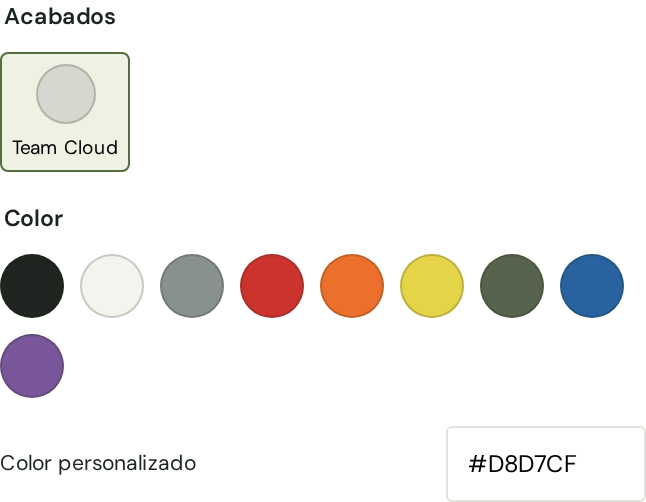
\includegraphics[width=4.8cm]{recursos/08-acabados.png}};\end{scope}
\hd{5.25}{1.96}{5.2}{19}{Ink}{PERSONALIZA}
\fill[Ink,rounded corners=4pt](11.05,1.65)rectangle(15.3,6.6);
\ico{save}{12.5}{6.1}{1.2}{Mint}
\node[anchor=north,inner sep=0]at(13.17,4.35){
\includegraphics[width=3.65cm]{recursos/13-renombrar.png}};
\hd{11.4}{2.17}{3.6}{19}{White}{RETOMA}
\source{Capturas reales de categorías, selección, apariencia y gestión de montajes. Cuenta de demostración eliminada.}
\finish\note{Muestra los módulos desde el punto de vista del usuario. El catálogo permite ubicar piezas y abrir fichas; la comparación complementa esa consulta. El configurador organiza posiciones por grupos, filtra alternativas y muestra acabados. Mis bicicletas conserva propuestas y permite continuar, renombrar o eliminar. Las imágenes son controles reales recortados para mantener el foco y evitar datos personales. La seguridad y administración completan estos módulos. Tiempo: 55 segundos. Las tres composiciones reúnen controles reales con distinta jerarquía visual; no recrean nuevas pantallas.}
\end{frame}

% 10. Demostración · montaje protagonista
\begin{frame}[plain]
\canvas{light}\header{09 / DEMOSTRACIÓN}{Elegir. Personalizar. Guardar.}
\begin{scope}\clip[rounded corners=4pt](.7,1.78)rectangle(10.4,6.65);\node[inner sep=0]at(5.55,4.3){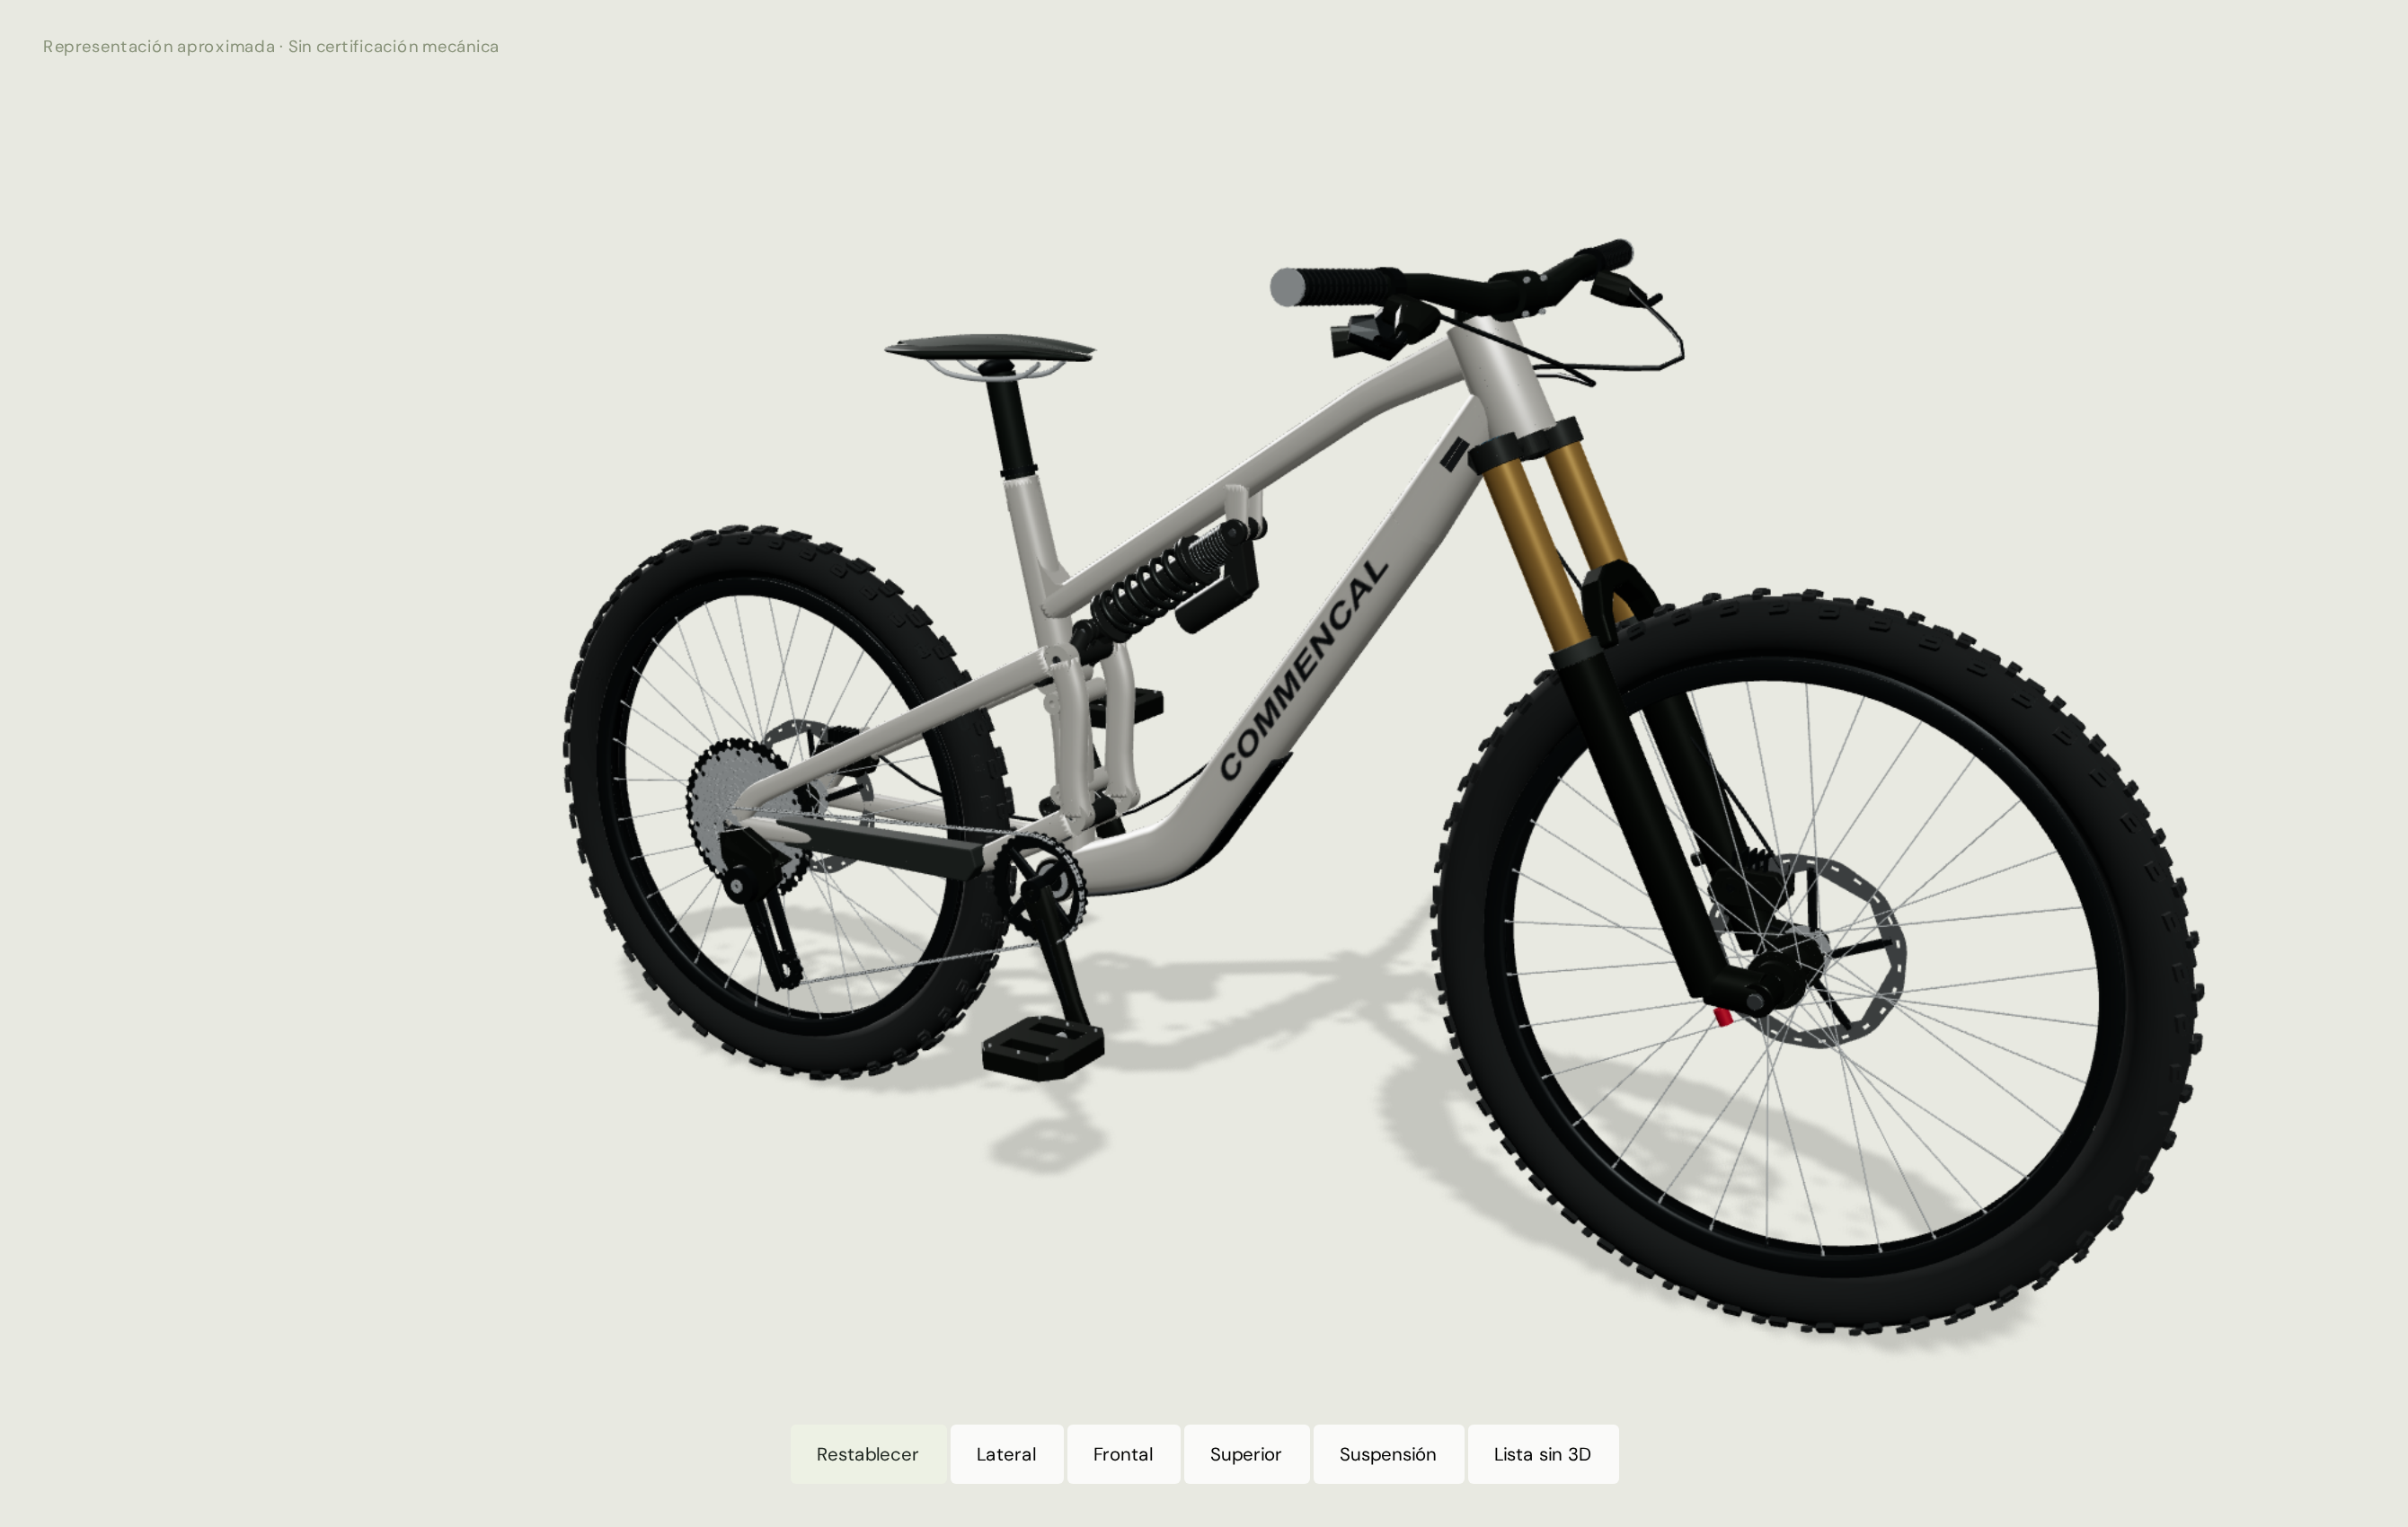
\includegraphics[width=10.4cm]{recursos/montaje-perspectiva.png}};\end{scope}
\draw[Line,line width=1pt](11.2,2.6)--(11.2,6.15);
\foreach \y/\n/\icon/\label in {6.25/1/layers/ELEGIR,4.65/2/paintbrush/PERSONALIZAR,3.05/3/save/GUARDAR}{
\fill[Paper](11.2,\y-.3)circle(.27);\node[font=\Body\bfseries\small,text=Accent]at(11.2,\y-.3){\n};\ico{\icon}{11.8}{\y}{.48}{Accent}\hd{12.5}{\y-.06}{2.8}{14}{Ink}{\label}}
\tx{.85}{1.48}{14.2}{9.5}{Accent}{\href{https://atlasmtb.netlify.app/}{\bfseries ABRIR DEMOSTRACIÓN\quad atlasmtb.netlify.app\quad \ensuremath{\nearrow}}}
\source{Elegir base \ensuremath{\rightarrow} cambiar una pieza o acabado \ensuremath{\rightarrow} guardar \ensuremath{\rightarrow} volver a abrir. Vista real en perspectiva; modelo visual aproximado.}
\finish\note{Antes de exponer, inicia sesión y prepara una composición de práctica; no proyectes contraseñas. Abre Bicicletas, selecciona Personalizar, muestra un grupo y cambia un acabado disponible. Explica que filtrar no reemplaza las piezas montadas. Revisa Avisos del montaje, asigna un nombre, guarda y espera Guardado. Abre Mis bicicletas y utiliza Continuar para demostrar la persistencia. Si falla la red, explica la misma secuencia con las capturas. Tiempo: unos 2 minutos. El montaje se muestra en perspectiva, capturado directamente del visor sin guardar cambios de catálogo.}
\end{frame}

% 11. Resultados · evidencia y límites
\begin{frame}[plain]
\canvas{dark}\header{10 / RESULTADOS}{Evidencia de funcionamiento}
\hd{.8}{6.8}{5}{58}{Mint}{487}
\tx{1}{4.68}{4.8}{11}{White}{pruebas correctas}
\tx{1}{4.12}{4.8}{8.5}{Dim}{2 omitidas}
\hd{6.1}{6.8}{4}{58}{Mint}{13}
\tx{6.25}{4.68}{4.6}{11}{White}{comprobaciones públicas}
\ico{globe}{12.2}{6.6}{1.2}{Mint}\hd{11.4}{4.68}{4.1}{24}{White}{HTTPS}
\tx{11.4}{3.8}{4.1}{9}{Dim}{Web publicada}
\draw[Line,opacity=.3](.85,3.3)--(15.15,3.3);
\foreach \x/\icon/\label in {1/save/Guardado y reapertura,6.15/shield-check/Aislamiento de cuentas,11.3/user-round/Google confirmado}{
\ico{\icon}{\x}{2.75}{.5}{Mint}\tx{\x+.72}{2.64}{3.9}{8.5}{White}{\label}}
\source{Fuente: informe/manual. Google: confirmación manual. Suite repetida con 2 trabajadores y límite de 15 s tras timeout inicial.}
\tx{.85}{1.48}{14.3}{7.2}{Dim}{Por evaluar: correo real, dispositivos físicos y experiencia con usuarios.}
\finish\note{No sumes como si fueran iguales las pruebas unitarias y las comprobaciones de navegador. El informe registra 487 correctas y dos omitidas después de repetir con dos trabajadores y un límite de 15 segundos, por un timeout inicial de cinco segundos. El manual completó 13 comprobaciones públicas y limpió su cuenta temporal; el informe también documenta aislamiento entre dos cuentas y conflicto de revisión. Google se confirmó manualmente. No afirmes entrega de correo validada, 30 FPS, Android físico o mejoras medidas en usuarios. Tiempo: 70 segundos.}
\end{frame}

% 12. Cierre · contribuciones y mejora
\begin{frame}[plain]
\canvas{dark}
\begin{scope}\clip(0,0)rectangle(6.2,9);\node[inner sep=0]at(3.1,4.6){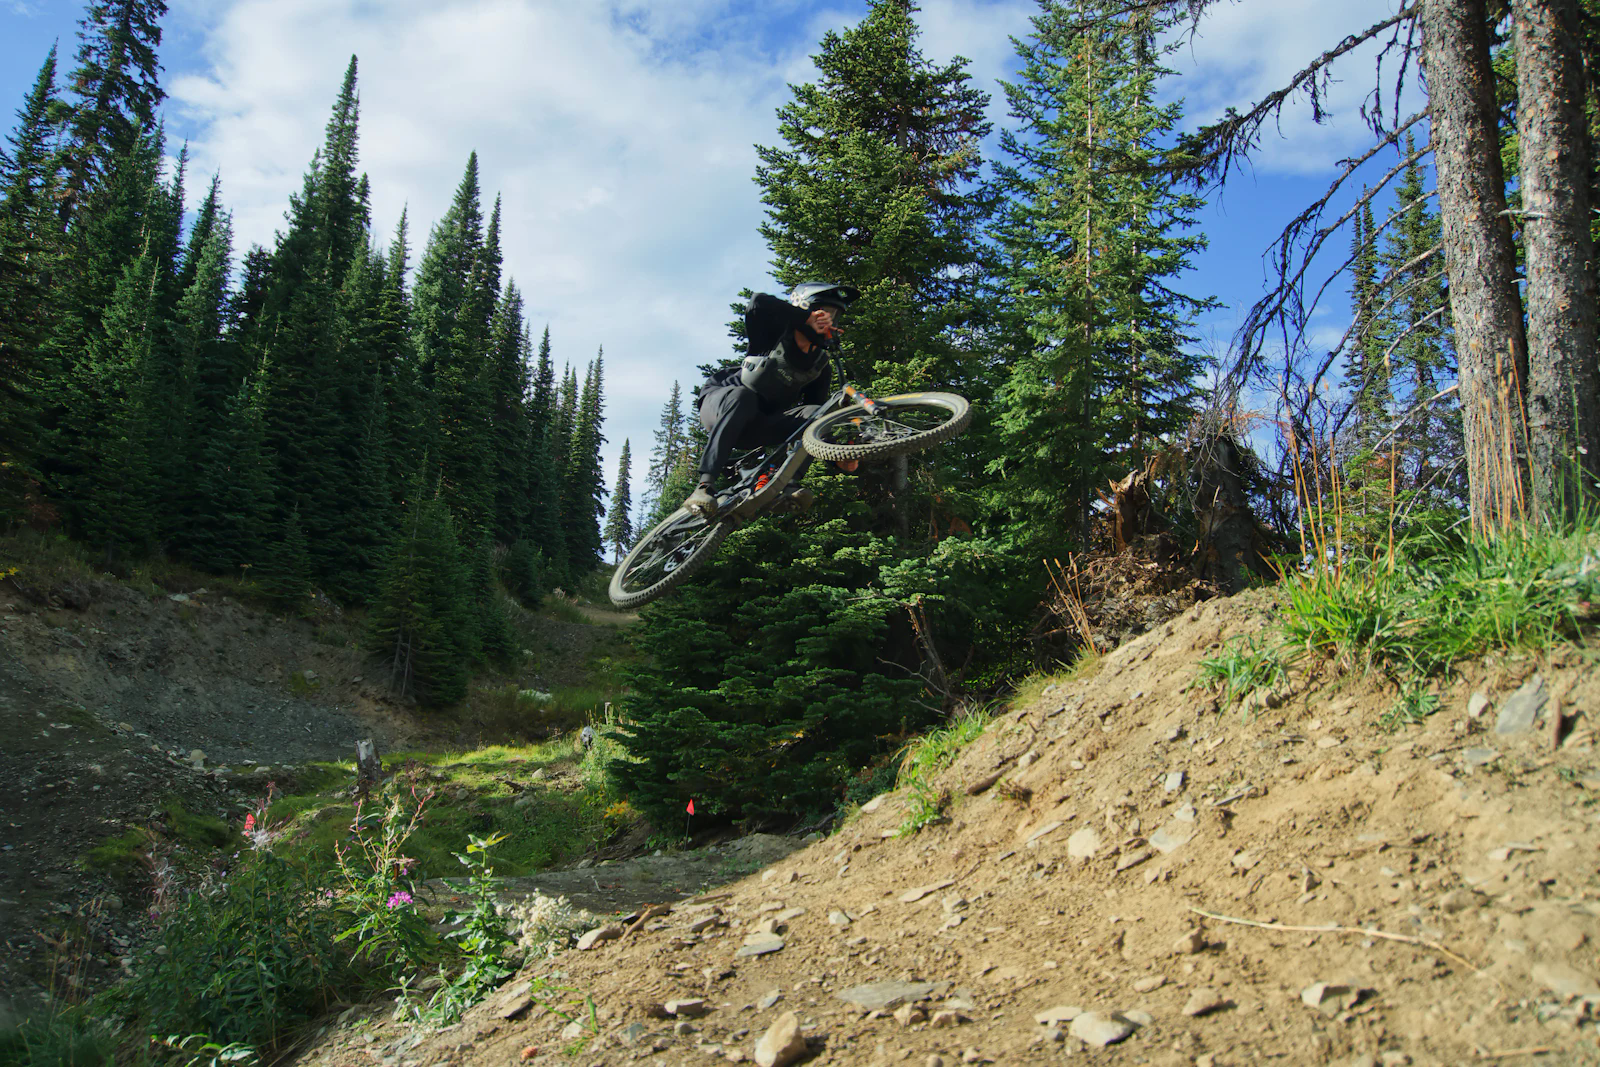
\includegraphics[height=9.8cm]{recursos/mtb-accion.png}};\fill[Night,opacity=.27](0,0)rectangle(6.2,9);\end{scope}
\tx{6.8}{8.45}{8.4}{7.5}{Mint}{11 / CONCLUSIONES}
\hd{6.75}{7.77}{8.6}{31}{White}{ELEGIR CON MÁS\\PERSPECTIVA}
\foreach \y/\label in {5.3/Consulta y configuración integradas,4.55/Montajes personales protegidos,3.8/Web operativa y comprobada}{\ico{circle-check}{6.85}{\y}{.38}{Mint}\tx{7.48}{\y-.07}{7.8}{10}{White}{\label}}
\tx{6.85}{2.75}{8.3}{7}{Mint}{SIGUIENTES MEJORAS}
\foreach \x/\icon/\label in {6.85/user-round/Usuarios,9.7/gauge/Rendimiento,12.55/database/Catálogo}{\ico{\icon}{\x}{2.15}{.5}{Mint}\tx{\x+.65}{2.02}{2.4}{7.7}{White}{\label}}
\tx{6.85}{1.38}{8.3}{10}{Mint}{\href{https://atlasmtb.netlify.app/}{atlasmtb.netlify.app\quad \ensuremath{\nearrow}}}
\tx{.65}{.96}{5.4}{5.2}{White}{Foto: Julien Kettmann / Unsplash}
\finish\note{Cierra con tres contribuciones: integrar consulta y configuración, conservar montajes personales y disponer de una web publicada con evidencia de recorridos. No afirmes una mejora porcentual porque no existe un estudio de usuarios que la mida. Como dificultades, menciona la diversidad de variantes y el mantenimiento de recursos visuales; las siguientes mejoras responden a esos límites. La utilidad es planificar; la validación física de piezas exige revisión especializada. Tiempo: 50 segundos.}
\end{frame}

\end{document}
